\section{}
\textit{For the two degree of freedom system shown, determine:}
\begin{figure}[H]
    \centering
    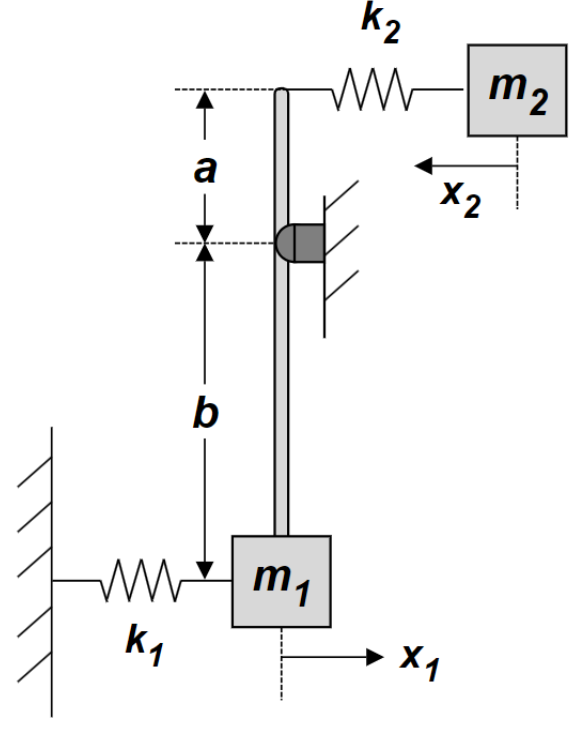
\includegraphics[width=0.5\textwidth]{Questions/Figures/Q1 Problem Diagram.png}
    \caption{Two degree of freedom system.}
    \label{fig:Q1}
\end{figure}

\subsection{}
\textit{The flexibility influence coefficients, starting from the definition.}

\begin{figure}[H]
    \centering
    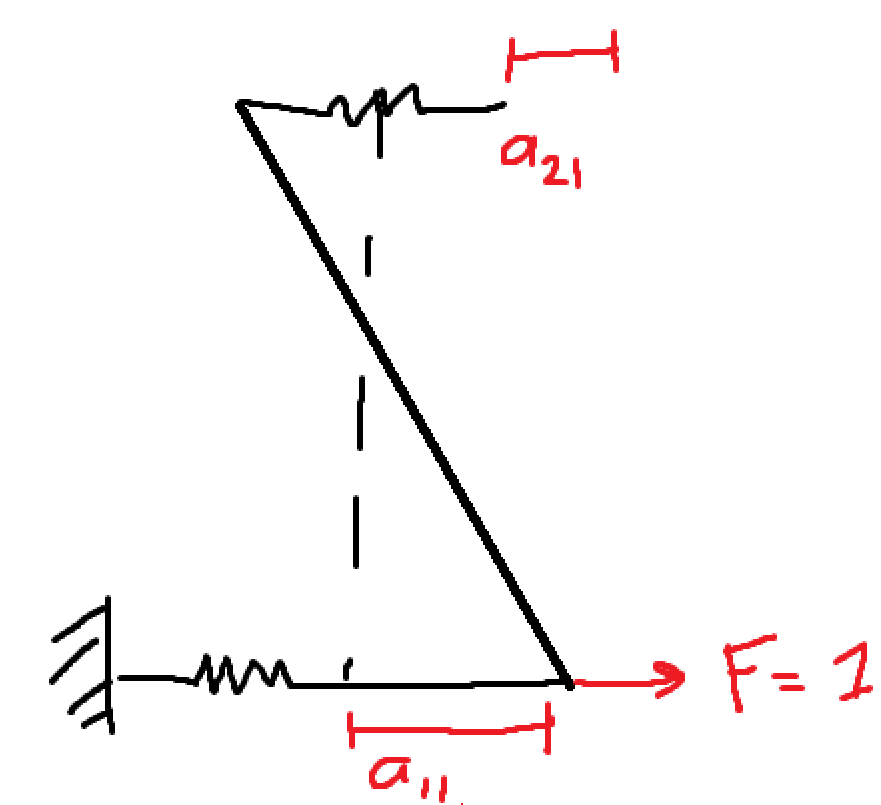
\includegraphics[width=0.5\textwidth]{Questions/Figures/Q1 a_i1.png}
    \caption{Resulting Displacements from Unit Force at Point 1.}
    \label{fig:Q1 a_i1}
\end{figure}
By definition, $a_{ij}$ is the displacement at point $i$ due to a unit force at point $j$, where all other coordinates are allowed to freely move. Starting with a unit force at point 1, the resulting displacements are shown in Figure \ref{fig:Q1 a_i1}. 

Since all other coordinates are allowed to freely move, the displacement of $a_{11}$ is then
\begin{align*}
    a_{11} &= \frac{1}{k_1}
\end{align*}
and the displacement of $a_{21}$ is pure rotation about the pin, so 
\begin{align*}
    a_{21} &= \frac{a}{b} a_{11} = \frac{a}{b} \frac{1}{k_1}
\end{align*}

\begin{figure}[H]
    \centering
    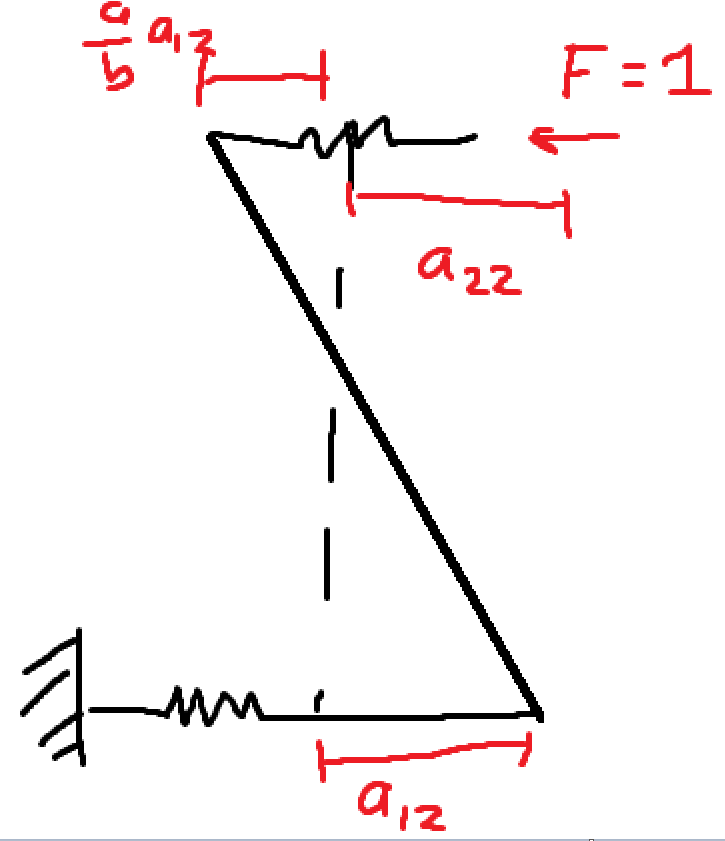
\includegraphics[width=0.5\textwidth]{Questions/Figures/Q1 a_i2.png}
    \caption{Resulting Displacements from Unit Force at Point 2.}
    \label{fig:Q1 a_i2}
\end{figure}
Next, with a unit force at point 2, the resulting displacements are shown in Figure \ref{fig:Q1 a_i2}. By Maxwell's Reciprocity Theorem, the displacement of $a_{12}$ is then
\begin{align*}
    a_{12} &= a_{21} = \frac{a}{b} \frac{1}{k_1}
\end{align*}
and the displacement of $a_{22}$ is
\begin{align*}
    a_{22} &= \frac{a}{b} a_{12} + \frac{1}{k_2} = \frac{a}{b} \frac{a}{b} \frac{1}{k_1} + \frac{1}{k_2}
\end{align*}

Then, the flexibility influence is 
\begin{empheq}[box=\fbox]{align*}
    \mathbf{A} &= \begin{bmatrix}
        a_{11} & a_{12} \\
        a_{21} & a_{22}
    \end{bmatrix} = \begin{bmatrix}
        \frac{1}{k_1} & \frac{a}{b} \frac{1}{k_1} \\
        \frac{a}{b} \frac{1}{k_1} & \frac{a^2}{b^2} \frac{1}{k_1} + \frac{1}{k_2}
    \end{bmatrix}
\end{empheq}

\subsection{}
\textit{The stiffness influence coefficients, starting from the definition.}

\begin{figure}[H]
    \centering
    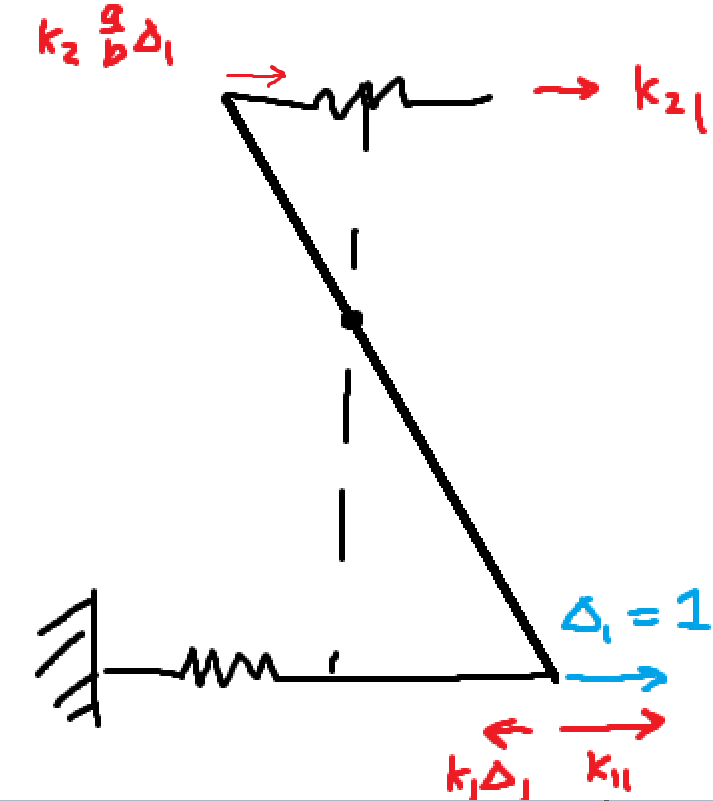
\includegraphics[width=0.5\textwidth]{Questions/Figures/Q1 k_i1.png}
    \caption{Resulting Forces from Unit Displacement at Point 1.}
    \label{fig:Q1 k_i1}
\end{figure}
By definition, $k_{ij}$ is the force at point $i$ due to a unit displacement at point $j$, where all other coordinates are held fixed. Starting with a unit displacement at point 1, the resulting forces are shown in Figure \ref{fig:Q1 k_i1}.

Since all other coordinates are held fixed, the force at $k_{11}$ can be determined by taking the moment about the pin, which gives,
\begin{align*}
    \circlearrowright \sum M_o :&=0 \\
    \implies k_{11} &= k_1 + \frac{a}{b} k_2
\end{align*}
and the force at $k_{21}$ is then,
\begin{align*}
    k_{21} &= -\frac{a}{b} k_{1} = -\frac{a}{b} k_1
\end{align*}

\begin{figure}[H]
    \centering
    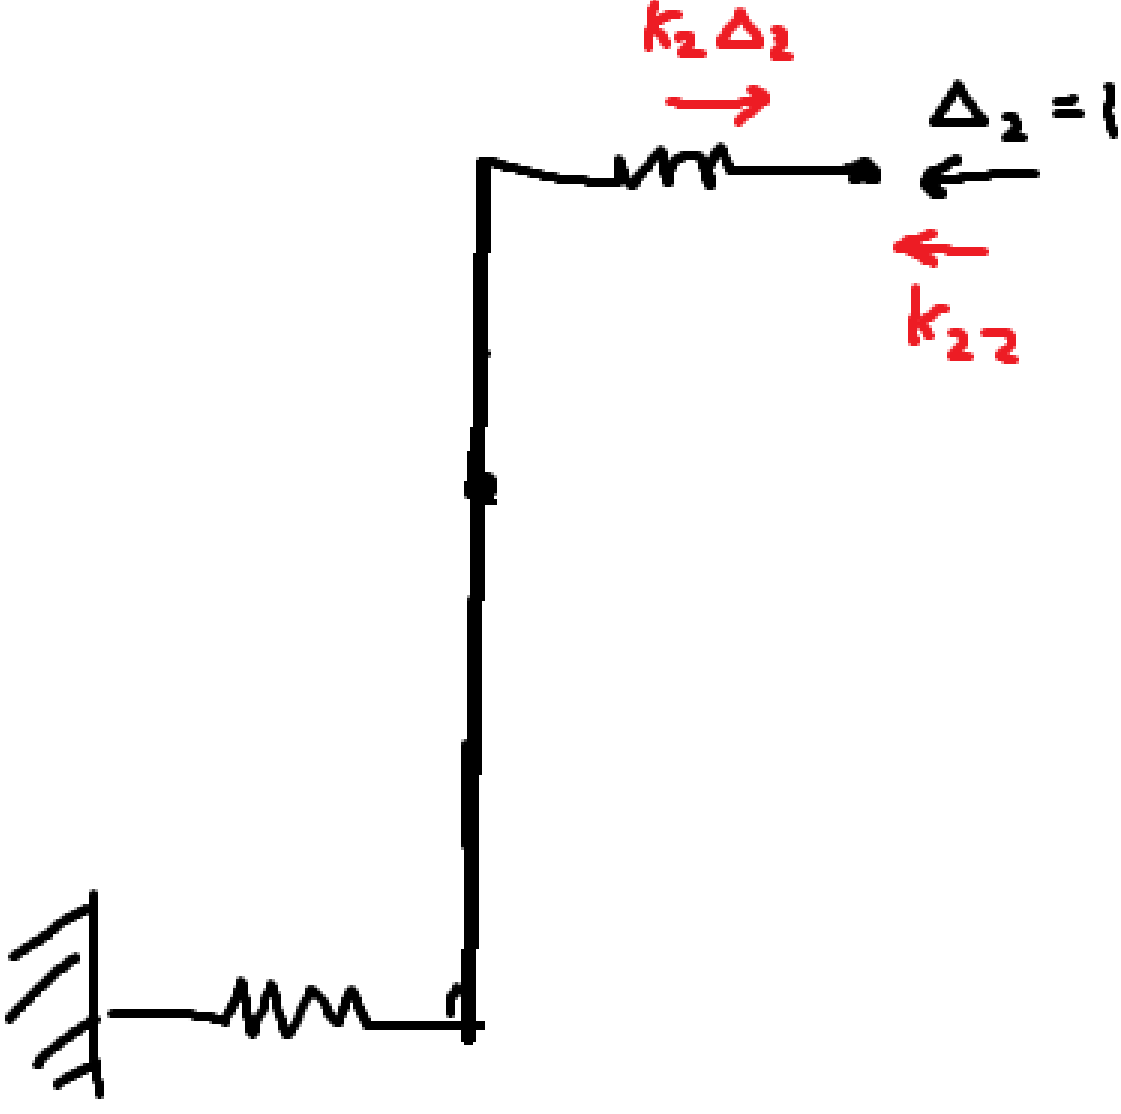
\includegraphics[width=0.5\textwidth]{Questions/Figures/Q1 k_i2.png}
    \caption{Resulting Forces from Unit Displacement at Point 2.}
    \label{fig:Q1 k_i2}
\end{figure}
Next, with a unit displacement at point 2, the resulting forces are shown in Figure \ref{fig:Q1 k_i2}. By Maxwell's Reciprocity Theorem, the force at $k_{12}$ is then,
\begin{align*}
    k_{12} &= k_{21} = -\frac{a}{b} k_1
\end{align*}
and the force at $k_{22}$ is then,
\begin{align*}
    k_{22} &= k_2
\end{align*}
    
Then, the stiffness influence is
\begin{empheq}[box=\fbox]{align*}
    \mathbf{K} &= \begin{bmatrix}
        k_{11} & k_{12} \\
        k_{21} & k_{22}
    \end{bmatrix} = \begin{bmatrix}
        k_1 + \frac{a}{b} k_2 & -\frac{a}{b} k_1 \\
        -\frac{a}{b} k_1 & k_2
    \end{bmatrix}
\end{empheq}

\subsection{}
\textit{If $k_1 = k$, $k_2 = 2k$, $m_2 = m_1 = m$, and $b = 2a$, the equations of motion are:}
\begin{align*}
    \begin{bmatrix}
        m & 0 \\
        0 & m
    \end{bmatrix} \begin{Bmatrix}
        \ddot{x}_1 \\
        \ddot{x}_2
    \end{Bmatrix} + \begin{bmatrix}
        \frac{3k}{2} & -k \\
        -k & 2k
    \end{bmatrix} \begin{Bmatrix}
        x_1 \\
        x_2
    \end{Bmatrix} = \begin{Bmatrix}
        0 \\
        0
    \end{Bmatrix}
\end{align*}
\textit{Determine the natural frequencies and mode shapes.}

By Matlab,
\begin{verbatim}
syms k m
M = [m 0; 0 m];
K = [3*k/2 -k; -k 2*k];
[V, D] = eig(inv(M)*K);
p = diag(D);
simplify(p)
simplify(V)

>> ans =
 
(k*(17^(1/2) + 7))/(4*m)
-(k*(17^(1/2) - 7))/(4*m)


>> ans =

[1/4 - 17^(1/2)/4, 17^(1/2)/4 + 1/4]
[               1,                1]
\end{verbatim}

Therefore,
\begin{empheq}[box=\fbox]{align*}
    p_1 &= \frac{k}{4m} \left(7 + \sqrt{17}\right) \\
    p_2 &= \frac{k}{4m} \left(7 - \sqrt{17}\right) \\
\end{empheq}
and
\begin{empheq}[box=\fbox]{align*}
    \{\Phi\}^{\textcircled{1}} &= \begin{bmatrix}
        \frac{1}{4} - \frac{\sqrt{17}}{4} \\
        1 
    \end{bmatrix} \\
    \{\Phi\}^{\textcircled{2}} &= \begin{bmatrix}
        \frac{1}{4} + \frac{\sqrt{17}}{4} \\
        1
    \end{bmatrix}
\end{empheq}